\documentclass[lettersize,journal]{IEEEtran}
\usepackage{amsmath,amsfonts}
\usepackage{algorithmic}
\usepackage{array}
\usepackage{graphicx}
\usepackage{booktabs}
\usepackage{mathtools}
\usepackage{stfloats}
\usepackage{url}
\usepackage{multirow}
\usepackage{threeparttable}
\usepackage[font=normalsize,labelfont=sf,textfont=sf]{subfig}
\usepackage{balance}

% For proper < and > symbols in text
\usepackage{textcomp}

\title{Trade-off Between Accuracy and Resources in CSI Feedback Compression}
\author{Your Name}

\begin{document}
\maketitle

\section{Trade-off Between Accuracy and Resources} 

CNNs have demonstrated superior performance in CSI compression tasks compared to compressive sensing methods. While numerous architectures have been proposed, deploying these models on mobile hardware presents significant challenges. Consequently, it becomes imperative to strike a balance between accuracy and resource constraints when considering the practical application of CSI feedback compression on user equipment with limited resources.

Most research in CSI feedback compression focuses on various designs of auto-encoders. A significant portion of the parameters and FLOPs in auto-encoder designs is attributed to the fully connected layer. Considering the CsiNet \cite{abe} architecture, initial measurements indicate a computational load of 5.6 million FLOPs and 2.1 million trainable parameters. Upon selective removal of the fully connected layers within the architecture, these metrics were reassessed, revealing a notable reduction. Specifically, the FLOPs decreased to 3.5 million, while the number of trainable parameters plummeted to 3400.

This analysis underscores a substantial optimization opportunity through the elimination of fully connected layers. Notably, the removal of these layers resulted in a reduction of approximately 37.5\% in FLOPs, indicating a significant computational burden alleviation. Moreover, the parameter count experienced a staggering decrease of over 99.8\%, illuminating the dominant role played by fully connected layers in parameter-heavy neural network architectures such as CsiNet \cite{abe}.

Additionally, kernel size in CNNs structure stands out as a crucial factor influencing the computational complexity of CNNs within the CsiNet \cite{abe} architecture. Initially set at (3,3), altering the kernel size to (7,7) prompts a significant shift in computational requirements. Specifically, this adjustment results in a notable increase, with FLOPs soaring to 20.3 million and the number of parameters remaining at 2.1 million.

This shift underscores the profound impact of kernel size on computational demands within CNNs architectures. Notably, enlarging the kernel size to (7,7) yields a substantial rise in FLOPs, escalating by approximately 362\%. Furthermore, the adjustment marginally affects the parameter count, increasing it by a modest 1.44\%.

These findings underscore the intricate interplay between kernel size and computational complexity in CNNs architectures such as CsiNet \cite{abe}. Such insights are valuable for optimizing network design to achieve desired performance outcomes while managing computational resources effectively.

CsiNet \cite{abe} achieves a parameter count under 1 million, while ACRNet \cite{abx} and CRNet \cite{abn} achieve superior Normalized Mean Square Error (NMSE) performance while maintaining a parameter count similar to CsiNet \cite{abe}. DS-NLCsiNet \cite{abq} achieves an NMSE near $-17$\,dB with nearly 10 million FLOPs and a parameter count similar to CsiNet. In contrast, Deep Decoder \cite{aby} and TransNet \cite{abz} have over 50 million FLOPs and 25\% and 30\% more parameters, respectively, compared to CsiNet (Figure \ref{fig:nmse-params} and \ref{fig:nmse-flops}).

\begin{figure}[!t]
  \centering
  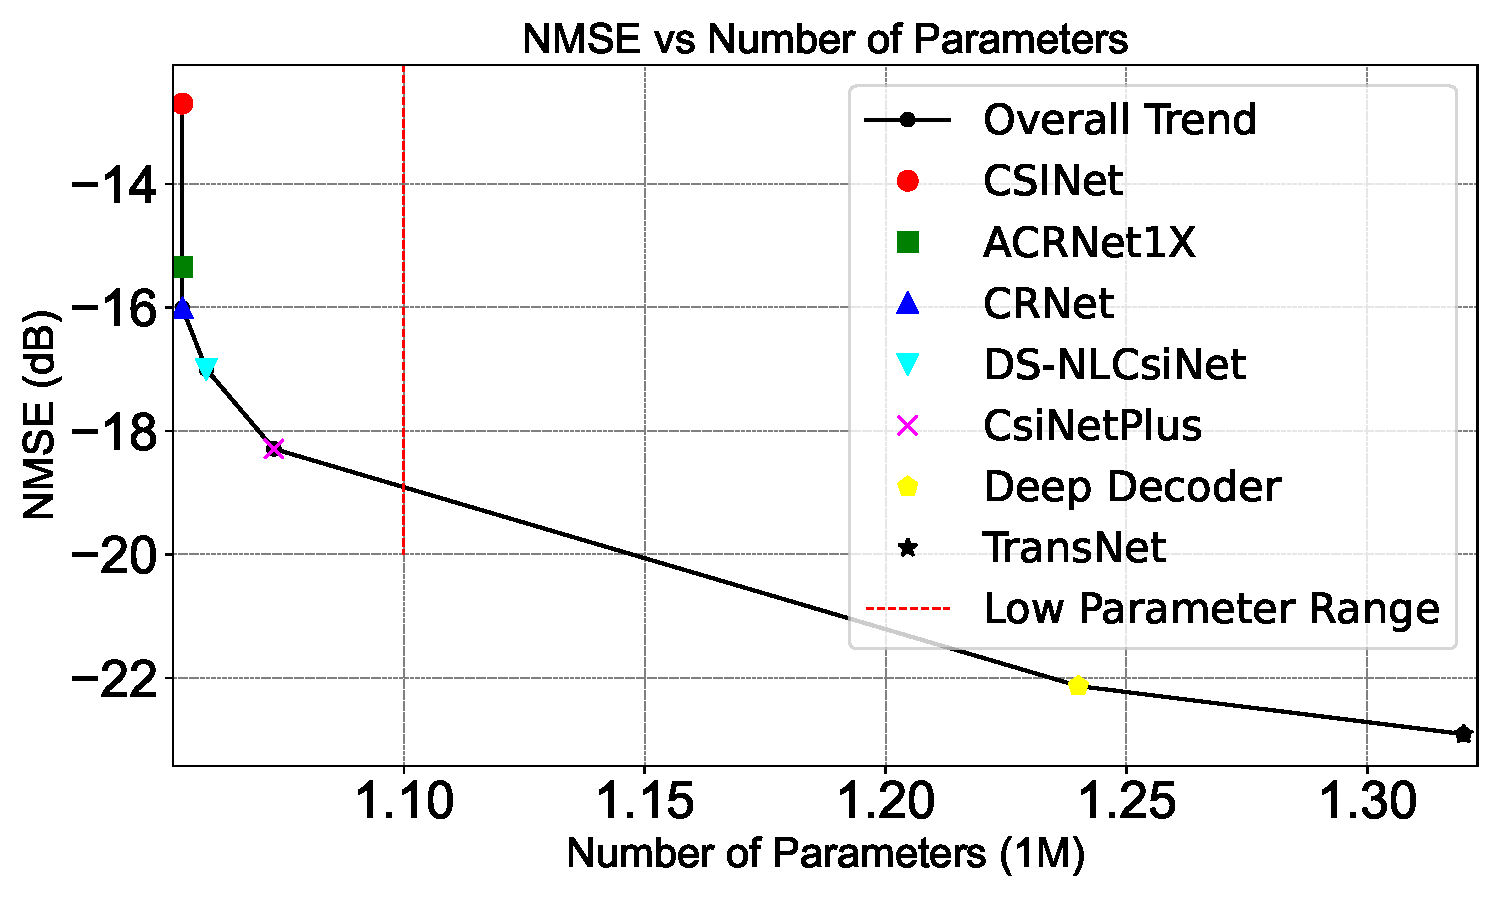
\includegraphics[width=0.45\textwidth]{NMSEvsNofparametters.pdf}
  \caption{NMSE vs Number of Parameters}
  \label{fig:nmse-params}
\end{figure}

\begin{figure}[!t]
  \centering
  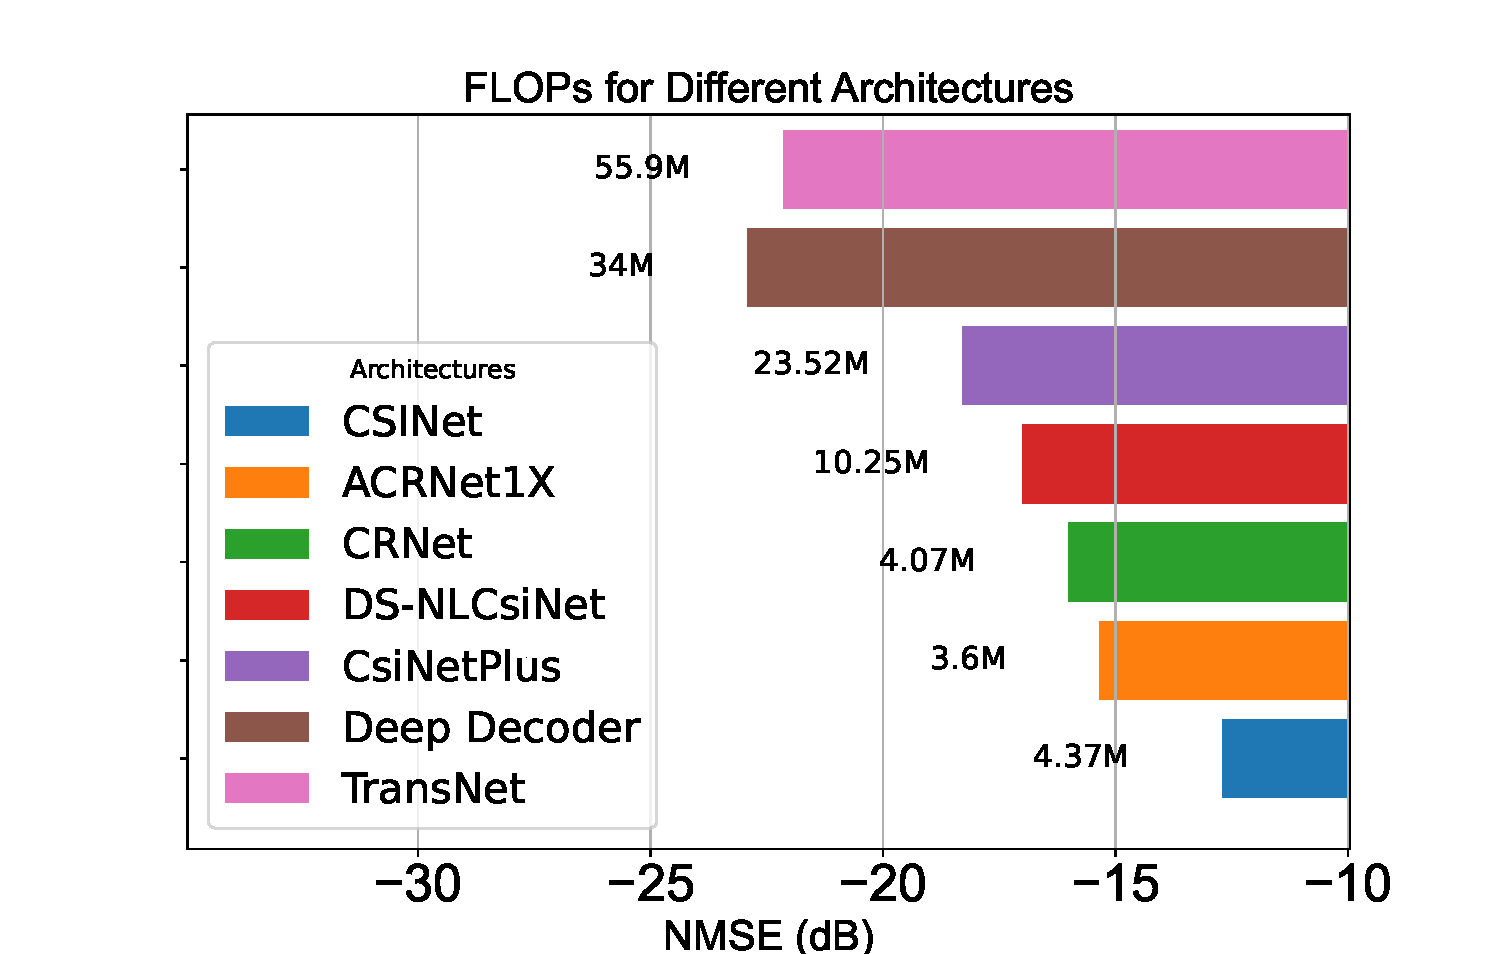
\includegraphics[width=0.45\textwidth]{NMSEvsFLOPs.pdf}
  \caption{NMSE vs FLOPs}
  \label{fig:nmse-flops}
\end{figure}

Many researchers primarily focus on increasing accuracy without considering the practical deployment of their proposed architectures. However, beyond addressing the imperfect channel, a challenge for evaluating the real performance of deep learning versus compressive sensing methods lies in considering storage constraints. Lu et al. \cite{abp} discuss the flexible deployment of their proposed architecture by adjusting kernel sizes for the convolutional neural network part of the auto-encoder and implementing network binarization for the fully connected layer. Lu et al. \cite{abp} also propose feature quantization for bitstream generation, replacing the feedback of floating-point numbers, which may not be feasible in digital communication systems.

As highlighted by Lu et al. \cite{abp}, adjusting kernel sizes can enhance spatial correlation extraction, particularly not beneficial for CSI matrices characterized by inherent randomness due to wireless channel conditions. Furthermore, Lu et al.'s introduction \cite{abp} of network binarization represents a novel approach, marking the first application of binary neural networks \cite{aaa1} in this domain.

Many studies in this field prioritize optimizing the NMSE, overlooking the practical implications of models in real-world scenarios involving imperfect channels in wireless communication. Factors such as short-term channel correlation and resource constraints are frequently overlooked, despite their considerable dependency on model runtime. The runtime of most models is heavily reliant on the Graphics Processing Unit (GPU) of the hardware on which these models are evaluated, and this runtime is proportional to the FLOPs. Most proposed models exhibit higher NMSE when considering a snapshot of CSI and assuming zero mobility of User Equipment (UE). To address this gap, we evaluate several state-of-the-art proposed models using the QuadriGa dataset \cite{abu}. Since most models are trained on the COST2100 \cite{abf} channel model, it's essential to consider its implications for generalization to real-world scenarios. We generate CSI samples while considering the mobility of UE, and we examine snapshots at various time intervals to assess the generalization capabilities of the proposed models. We quantified the number of FLOPs and parameters required for User Equipment (UE) in Table \ref{table:methods_params}. Notably, most proposed models demand at least one million parameters, emphasizing the need to consider resource limitations and computational efficiency alongside NMSE optimization in model design. One of our proposed approaches to mitigate the high parameter count is to utilize alternative compression techniques, acknowledging that it may result in a slight loss of accuracy. If a significant decrease in accuracy occurs, it will demonstrate the dependence of these models on the fully connected network.

\begin{table}[htb]
  \centering
  \caption{Methods Parameters Comparison}
  \label{table:methods_params}
  \begin{tabular}{lcc}
    \toprule
    \textbf{Method} & \textbf{UE Params} & \textbf{UE FLOPs} \\
    \midrule
    CsiNet & 1052K & 1094K \\
    CRNet & 1049K & 1235K \\
    ACRNet-1x & 1049K & 1235K \\
    CsiNetPlus & 1049K & 1462K \\
    TransNet & 2381K & 1054K \\
    \bottomrule
  \end{tabular}
\end{table}

\begin{thebibliography}{00}
\bibitem{abe} C. Wen et al., ``Deep Learning for Massive MIMO CSI Feedback,'' \emph{IEEE Wireless Commun. Lett.}, vol. 7, no. 5, pp. 748--751, 2018.
\bibitem{abx} Z. Lu et al., ``Binarized Aggregated Network With Quantization,'' \emph{IEEE Trans. Wireless Commun.}, vol. 21, no. 7, pp. 5514--5525, 2022.
\bibitem{abn} Z. Lu et al., ``Multi-resolution CSI Feedback With Deep Learning,'' \emph{ICC}, pp. 1--6, 2020.
\bibitem{abq} X. Yu et al., ``DS-NLCsiNet: Exploiting Non-Local Neural Networks,'' \emph{IEEE Commun. Lett.}, vol. 24, no. 12, pp. 2790--2794, 2020.
\bibitem{aby} A. Chakma et al., ``Deep Decoder CsiNet for FDD Massive MIMO,'' \emph{IEEE Wireless Commun. Lett.}, vol. 12, no. 12, pp. 2073--2077, 2023.
\bibitem{abz} Y. Cui et al., ``TransNet: Full Attention Network for CSI Feedback,'' \emph{IEEE Wireless Commun. Lett.}, vol. 11, no. 5, pp. 903--907, 2022.
\bibitem{abp} Z. Lu et al., ``Binary Neural Network Aided CSI Feedback,'' \emph{IEEE Wireless Commun. Lett.}, 2020.
\bibitem{aaa1} M. Nagel et al., ``A White Paper on Neural Network Quantization,'' \emph{arXiv:2106.08295}, 2021.
\bibitem{abu} F. Burkhardt et al., ``QuaDRiGa: A MIMO Channel Model,'' \emph{EuCAP}, pp. 1274--1278, 2014.
\bibitem{abf} L. Liu et al., ``The COST 2100 MIMO Channel Model,'' \emph{IEEE Wireless Commun.}, vol. 19, pp. 92--99, 2012.
\end{thebibliography}

\end{document}